	\chapter{Kravspecifikation}
	
	\section{Systembeskrivelse}
			Systemet består af en database med brugeradgang via web- eller Android applikation.
			Databasen indeholder brugere, sager og data om lysreguleringerne.
			En sag indeholder en fejlkode, kommentarfelt, mulighed for upload af billede og status.
			Der er fire tilstande af status som en sag kan have: Oprettet, Påbegyndt, Afventer og Afsluttet. På figur \ref{fig:OversigtSystembeskrivelse} beskrives sammenhængen mellem enhederne i systemet.
			
			\begin{figure}[H]
				\centering
				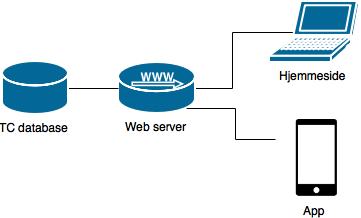
\includegraphics[width=0.6\linewidth]{Kravspecifikation/Oversigtoversystem}
				\caption{Oversigt over systemet}
				\label{fig:OversigtSystembeskrivelse}
			\end{figure}
			
			Systemet skal kunne oprette sager, når Randers Kommune modtager en fejlmeddelelse.
			Disse skal kunne tilgås af Strøm Hansen og Randers Kommune gennem den ønskede bruger adgang via PC eller smartphone.
			Systemet skal kunne notificere Strøm Hansen og Randers Kommune, når der foretages reparationer på en given sag. Notifikationen vil være igennem enten Android applikationen, e-mail eller SMS.
			Montørerne bliver tildelt et personligt log ind, som skal bruges når de foretager en reparation på en given sag.
			Montøren har mulighed for at ændre status på en oprettet sag. Derudover har montøren mulighed for at uploade relevante billeder og skrive kommentarer til reparationen.
			Systemet har en log, som indeholder en liste over alle sager, hvori det vil være muligt at søge og sortere i.
			
			
			\section{Afgrænsning}
			Projektet har en naturlig begrænsning i form af den korte tid fra idé til produkt, som er gældende for semesterprojekter. 
			
			Web applikationen vil blive udviklet med ASP.NET MVC. 
			Smartphone applikationen vil blive udviklet til Android. Til Android anvendes Xamarin, det muliggør at skrive i C\#.
			Både web- og android applikationen vil have et grafisk brugergrænseflade (GUI). Web applikationen vil kunne skalere opløsningen alt efter hvilken enhed applikationen tilgås fra.\\

\section{User stories} \label{sec:UserStories}
Følgende er en beskrivelse af de aktuelle krav stillet til projektet. De er alle opstillet som user stories. User stories er korte beskrivelser af funktionalitet, som står på en fast form. De er let læselige og har værdi for både personer direkte involveret i projektet og udefrakommende, som skal opnå en idé om kravene til projektet. 

\subsection{Aktør kontekst diagram}\label{sec:aktor}
På figur \ref{fig:AktorKontekst} ses aktør kontekst diagrammet for Traffic Control. Diagrammet viser hvilke aktør der interagere med systemet.
	\begin{figure}[H]
		\centering
		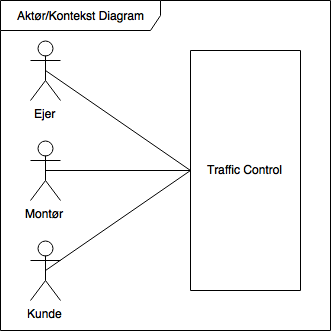
\includegraphics[width=0.4\linewidth]{Kravspecifikation/AktorDiagram}
		\caption{Aktør kontekst diagram for Traffic Control}
		\label{fig:AktorKontekst}
	\end{figure}


\textbf{Beskrivelse af termer anvendt i kravspecifikationen}\\
Bruger = Kunde, Montør og Ejer\\
\indent Brugeren er en fælles betegnelse for alle aktør, dvs. alle aktører er involveret når "Brugeren" bliver nævnt. \\
Kunde = Randers kommune\\
Ejer = Strøm Hansen\\
Montør = Ansat ved Strøm Hansen, som udfører opgave\\
Sag = En fejl på systemet, som kræver en handling. Mulighed for at indeholde status, kommentarer, billeder, personer der er tilknyttet, dato mv.\\
Driftstatus = Status for en sag. Kan være: "Oprettet", "Påbegyndt", "Afsluttet" og "Afventer"\\
Log = Liste over sager\\

\subsection{User stories beskrevet med Gherkin}
Til beskrivelse af user stories er Gherkin-syntaksen valgt, hvor stories 
kan skrives på et flydende sprog, mens de er testbare.\cite{Gherkin} Dette kaldes også et Business-Readable Domain  
Specific Language. En særlig fordel ved anvendelsen af syntaksen er at den er opstiller kravene så de er særligt testbare, hvilket medfører at kravene for test af features er skrevet i user stories.
 Gherkin anvender nøgleord (i det flg. afsnit 
markeret med blåt), som hver især har en funktion i beskrivelsen af hver 
user story.  \vspace{0.2 cm}\\
Første del af en egenskab indeholder en beskrivelse af forretningsdomænet. 
Formatet i	dette afsnit vælges frit. Det anbefales, at man anvender et 
system, hvor der som minimum svares på hvilke aktører der har et behov, hvad 
behovet består af og hvorfor aktører har dette behov. En tre trins user 
story opfylder dette krav og opstilles med tre 
sætninger. Første sætning svarer på hvilken aktør, eller aktører der har
behovet. Dernæst svarer man på hvad det konkret er at aktøreren ønsker at 
opnå. Den tredje sætning beskriver aktørens motivation for at anvende 
funktionaliteten\\
Samtlige nøgleord beskrives nedenfor:

\large{\textbf{Givet}}\\
Disse trin definerer tilstande og datastrukturer som anvendes i de 
efterfølgende trin og scenarier.\\
\large{\textbf{Når}}\\
Disse trin beskriver handlinger som ændrer Scenariets tilstand. Dette kan 
være handlinger	foretaget af aktøreren og/eller systemet.\\
\large{\textbf{Så}}\\
Disse trin definerer udfaldet af forudgående handlinger i et givet 
scenarie. Alle scenarier skal afsluttes ved at definere et det forventede 
udfald i et eller flere "Så"trin.\\
\large{\textbf{Scenarier}}\\
Scenarier er samlinger af trin som definerer de funktionelle krav til 
forløb. Første scenarie i en egenskab dækker hovedfunktionaliteten. De 
efterfølgende scenarier dækker fejlhåndteringer og alternative scenarier.\\
\large{\textbf{Baggrund}}\\
Baggrund er en særlig type scenarie som udføres inden hvert af de 
efterfølgende scenarier	i egenskaben. Systemets tilstand og preconditions 
beskrives under overskriften "Baggrund" efterfulgt af et kolon og 
linjeskift. Herefter listes alle de data, tilstande og handlinger som udgør 
systemets tilstand inden samtlige af de efterfølgende Scenarier kan	udføres.


\subsubsection{Log ind}
\textbf{\textsc{\textcolor{RoyalBlue} {Egenskab:} Log-in på applikationen}} \\
Som bruger\\
Ønsker jeg at kunne logge ind på applikationen\\
For at kunne benytte applikationen\\

\textbf{\textsc{\color{RoyalBlue}Baggrund:}}\\
\textcolor{RoyalBlue}{Givet} følgende eksisterende profil\\
\begin{tabular}{| l | l | l | l |}
	\textbf{fornavn} & \textbf{efternavn} & \textbf{e-mail} & \textbf{kode} \\
	Jacob & Testbruger & jacob@mail.dk & letmein\\
\end{tabular}
\newline \newline
\textcolor{RoyalBlue}{Og} "Jacob" er ikke allerede logget ind i systemet\\
\textcolor{RoyalBlue}{Og} han har navigeret til applikationens log-in side\\

\clearpage

\textbf{\textsc{\textcolor{RoyalBlue}{Scenarie:}} Log ind med korrekte oplysninger - Android applikation}\\
\textcolor{RoyalBlue}{Når} "Jacob" indtaster sin mail og kode i de korrekte tekstfelter\\
\textcolor{RoyalBlue}{Og} han trykker på log-in knappen\\
\textcolor{RoyalBlue}{Så} navigeres han til applikationens forside\\

\textbf{\textsc{\textcolor{RoyalBlue}{Scenarie:}} Log ind med korrekte oplysninger - Web applikation}\\
\textcolor{RoyalBlue}{Når} "Jacob" indtaster sin mail og kode i de korrekte tekstfelter\\
\textcolor{RoyalBlue}{Og} han trykker på log-in knappen\\
\textcolor{RoyalBlue}{Så} navigeres han til applikationens forside\\

\textbf{\textsc{\textcolor{RoyalBlue}{Scenarie:}} Log ind med forkerte oplysninger - Android applikation}\\
\textcolor{RoyalBlue}{Når} "Jacob" indtaster følgende oplysninger:\\
\begin{tabular}{| l | l |}
	\textbf{e-mail} & \textbf{kode}\\
	jacob@mail.dk & 123\\
\end{tabular}
\newline \newline
\textcolor{RoyalBlue}{Og} han trykker på log-in knappen\\
\textcolor{RoyalBlue}{Så} informeres han om, at der er indtastet forkerte oplysninger\\
\textcolor{RoyalBlue}{Og} han bliver på log-in siden\\


\textbf{\textsc{\textcolor{RoyalBlue}{Scenarie:}} Log ind med forkerte oplysninger - Web applikationen}\\
\textcolor{RoyalBlue}{Når} "Jacob" indtaster følgende oplysninger:\\
\begin{tabular}{| l | l |}
	\textbf{e-mail} & \textbf{kode}\\
	jacob@mail.dk & 123\\
\end{tabular}
\newline \newline
\textcolor{RoyalBlue}{Og} han trykker på log-in knappen\\
\textcolor{RoyalBlue}{Så} informeres han om, at der er indtastet forkerte oplysninger\\
\textcolor{RoyalBlue}{Og} han bliver på log-in siden\\

\subsubsection{Opret bruger} \label{sec:USOpretBruger}
\textbf{\textsc{\textcolor{RoyalBlue}{Egenskab:} Opret bruger på applikationen}} \\
Som ejer\\
Ønsker jeg at kunne oprette bruger på applikationen\\
For at kunne give montører samt kunder adgang til systemet\\

\textcolor{RoyalBlue}{\textbf{\textsc{Baggrund:}}}\\
\textcolor{RoyalBlue}{Givet} at ejeren "Rasmus" er logget ind som administrator \\
\textcolor{RoyalBlue}{Og} han vil oprette en bruger med følgende oplysninger:\\
\begin{tabular}{| l | l |}
	\textbf{e-mail} & \textbf{kode} \\
	morten@randers.dk & solskin\\
\end{tabular}
\newline \newline
\textcolor{RoyalBlue}{Og} han er navigeret til indstillinger for at oprette brugere\\

\textbf{\textsc{\textcolor{RoyalBlue}{Scenarie:}} Opret bruger med bruger-rettigheder - Android applikation}\\
\textcolor{RoyalBlue}{Når} "Rasmus" indtaster mail, kode, telefonnummer, 
fornavn og efternavn \\
\textcolor{RoyalBlue}{Og} vælger brugerrettigheder til Bruger\\
\textcolor{RoyalBlue}{Og} trykker på opret bruger-knappen\\
\textcolor{RoyalBlue}{Så} oprettes den nye bruger\\
\textcolor{RoyalBlue}{Og} den nye bruger kan logge ind\\

\textbf{\textsc{\textcolor{RoyalBlue}{Scenarie:}} Opret bruger med montør-rettigheder - Android applikation}\\
\textcolor{RoyalBlue}{Når} "Rasmus" indtaster mail, kode, telefonnummer, 
fornavn og efternavn \\
\textcolor{RoyalBlue}{Og} vælger brugerrettigheder til Montør\\
\textcolor{RoyalBlue}{Og} trykker på opret bruger-knappen\\
\textcolor{RoyalBlue}{Så} oprettes den nye bruger\\
\textcolor{RoyalBlue}{Og} den nye bruger kan logge ind\\

\textbf{\textsc{\textcolor{RoyalBlue}{Scenarie:}} Opret bruger med Admin-rettigheder - Android applikation}\\
\textcolor{RoyalBlue}{Når} "Rasmus" indtaster mail, kode, telefonnummer, 
fornavn og efternavn \\
\textcolor{RoyalBlue}{Og} vælger brugerrettigheder til Adminstrator\\
\textcolor{RoyalBlue}{Og} trykker på opret bruger-knappen\\
\textcolor{RoyalBlue}{Så} oprettes den nye bruger\\
\textcolor{RoyalBlue}{Og} den nye bruger kan logge ind\\

\textbf{\textsc{\textcolor{RoyalBlue}{Scenarie:}} Opret bruger med bruger-rettigheder - Web applikation}\\
\textcolor{RoyalBlue}{Når} "Rasmus" indtaster mail, kode, telefonnummer, 
fornavn og efternavn \\
\textcolor{RoyalBlue}{Og} vælger brugerrettigheder til Bruger\\
\textcolor{RoyalBlue}{Og} trykker på opret bruger-knappen\\
\textcolor{RoyalBlue}{Så} oprettes den nye bruger\\
\textcolor{RoyalBlue}{Og} den nye bruger kan logge ind\\

\textbf{\textsc{\textcolor{RoyalBlue}{Scenarie:}} Opret bruger med montør-rettigheder - Web applikation}\\
\textcolor{RoyalBlue}{Når}"Rasmus" indtaster mail, kode, telefonnummer, 
fornavn og efternavn \\
\textcolor{RoyalBlue}{Og} vælger brugerrettigheder til Montør\\
\textcolor{RoyalBlue}{Og} trykker på opret bruger-knappen\\
\textcolor{RoyalBlue}{Så} oprettes den nye bruger\\
\textcolor{RoyalBlue}{Og} den nye bruger kan logge ind\\

\textbf{\textsc{\textcolor{RoyalBlue}{Scenarie:}} Opret bruger med Admin-rettigheder - Web applikation}\\
\textcolor{RoyalBlue}{Når} "Rasmus" indtaster mail, kode, telefonnummer, 
fornavn og efternavn \\
\textcolor{RoyalBlue}{Og} vælger brugerrettigheder til Admin\\
\textcolor{RoyalBlue}{Og} trykker på opret bruger-knappen\\
\textcolor{RoyalBlue}{Så} oprettes den nye bruger\\
\textcolor{RoyalBlue}{Og} den nye bruger kan logge ind\\


\subsubsection{Ændring af brugeroplysninger}
\textbf{\textsc{\textcolor{RoyalBlue}{Egenskab:} Ændring af brugeroplysninger}}\\
Som bruger\\
Ønsker jeg at kunne ændre brugeroplysninger\\
For at have aktuelle oplysninger på applikationen\\

\textsc{\textcolor{RoyalBlue}{\textbf{Baggrund:}}}\\
\textcolor{RoyalBlue}{Givet} at "Cecilie" er logget ind\\
\textcolor{RoyalBlue}{Og} hun har følgende nuværende oplysninger:\\
\begin{tabular}{| l | l | l | l |}
	\textbf{fornavn} & \textbf{efternavn} & \textbf{kodeord} & \textbf{notifikationsindstillinger} \\
	Cecilie & Testbruger & paris & Kun e-mail\\
\end{tabular}
\newline \newline
\textcolor{RoyalBlue}{Og} at hun vil ændre indstillingerne til følgende:\\
\begin{tabular}{| l | l | l | l |}
	\textbf{fornavn} & \textbf{efternavn} & \textbf{kodeord} & \textbf{notifikationsindstillinger} \\
	Cille & TestTest & london & SMS og e-mail\\
\end{tabular}
\newline \newline
\textcolor{RoyalBlue}{Og} at hun er navigeret til indstillinger\\

\textbf{\textsc{\textcolor{RoyalBlue}{Scenarie:}} Ændr kode - Android applikation}\\
\textcolor{RoyalBlue}{Når} "Cecilie" indtaster "paris" i kodefeltet "Gammel adgangskode"\\
\textcolor{RoyalBlue}{Og} hun skriver "london" i "Ny adgangskode" og "Bekræft ny adgangskode"\\
\textcolor{RoyalBlue}{Og} hun trykker på gem oplysninger\\
\textcolor{RoyalBlue}{Så} gemmes oplysningerne\\
\textcolor{RoyalBlue}{Og} hun informeres om at ændringerne er gemt\\

\textbf{\textsc{\textcolor{RoyalBlue}{Scenarie:}} Ændr for- og efternavn - Android applikation}\\
\textcolor{RoyalBlue}{Når} "Cecilie" indtaster nyt for- og efternavn i de korrekte tekstfelter\\
\textcolor{RoyalBlue}{Og} hun trykker på ok\\
\textcolor{RoyalBlue}{Så} gemmes oplysningerne\\
\textcolor{RoyalBlue}{Og} hun kan se at ændringerne er gemt\\

\textbf{\textsc{\textcolor{RoyalBlue}{Scenarie:}} Ændr telefonnummer - Android applikation}\\
\textcolor{RoyalBlue}{Når} "Cecilie" indtaster "87654321" i det korrekte tekstfelt\\
\textcolor{RoyalBlue}{Og} hun trykker på ok\\
\textcolor{RoyalBlue}{Så} gemmes oplysningerne\\
\textcolor{RoyalBlue}{Og} hun kan se at ændringerne er gemt\\

\textbf{\textsc{\textcolor{RoyalBlue}{Scenarie:}} Ændr notifikationsindstillinger - Android applikation}\\
\textcolor{RoyalBlue}{Når} "Cecilie" vælger sætte flueben i SMS-feltet\\
\textcolor{RoyalBlue}{Så} kan hun se et flueben komme til syne\\
\textcolor{RoyalBlue}{Og} ændringerne er derved gemt\\

\textbf{\textsc{\textcolor{RoyalBlue}{Scenarie:}} Ændr kode - Web applikation}\\
\textcolor{RoyalBlue}{Når} "Cecilie" indtaster "paris" i kodefeltet\\
\textcolor{RoyalBlue}{Og} hun skriver "london" i de to ny-kode tekstfelter\\
\textcolor{RoyalBlue}{Og} hun trykker på gem oplysninger\\
\textcolor{RoyalBlue}{Så} gemmes oplysningerne\\
\textcolor{RoyalBlue}{Og} hun informeres om at ændringerne er gemt\\

\textbf{\textsc{\textcolor{RoyalBlue}{Scenarie:}} Ændr for- og efternavn - Web applikation}\\
\textcolor{RoyalBlue}{Når} "Cecilie" indtaster nyt for- og efternavn i de korrekte tekstfelter\\
\textcolor{RoyalBlue}{Og} hun trykker på gem oplysninger\\
\textcolor{RoyalBlue}{Så} gemmes oplysningerne\\
\textcolor{RoyalBlue}{Og} hun informeres om at ændringerne er gemt


\textbf{\textsc{\textcolor{RoyalBlue}{Scenarie:}} Ændr telefonnummer - Web applikation}\\
\textcolor{RoyalBlue}{Når} "Cecilie" indtaster "87654321" i det korrekte tekstfelt\\
\textcolor{RoyalBlue}{Og} hun trykker på gem oplysninger\\
\textcolor{RoyalBlue}{Så} gemmes oplysningerne\\
\textcolor{RoyalBlue}{Og} hun informeres om at ændringerne er gemt\\

\textbf{\textsc{\textcolor{RoyalBlue}{Scenarie:}} Ændr notifikationsindstillinger - Web applikation}\\
\textcolor{RoyalBlue}{Når} "Cecilie" vælger sætte flueben i SMS-feltet\\
\textcolor{RoyalBlue}{Og} hun trykker på gem oplysninger\\
\textcolor{RoyalBlue}{Så} gemmes oplysningerne\\
\textcolor{RoyalBlue}{Og} hun informeres om at ændringerne er gemt\\

\subsubsection{Opret en sag}\label{sec:USOpretSag}
\textbf{\textsc{\textcolor{RoyalBlue}{Egenskab:} Opret en sag}}\\
Som ejer eller montør\\
Ønsker jeg at kunne oprette en sag\\
For kunne lave en fejlmelding på et givent lyskryds\\

\textsc{\textcolor{RoyalBlue}{\textbf{Baggrund:}}}\\
\textcolor{RoyalBlue}{Givet} at "Søren" er logget ind\\
\textcolor{RoyalBlue}{Og} han har følgende nuværende oplysninger:\\
\begin{tabular}{| l | l |}
	\textbf{fornavn} & \textbf{rolle} \\
	Søren & Ejer eller Montør\\
\end{tabular}
\clearpage

\textbf{\textsc{\textcolor{RoyalBlue}{Scenarie:}} Opret en sag - Android applikation}\\
\textcolor{RoyalBlue}{Når} Søren vælger "Opret Sag"\\
\textcolor{RoyalBlue}{Og} han har valgt hvilken installation det drejer sig om\\
\textcolor{RoyalBlue}{Og} han har valgt hvem der har anmeldt skaden\\
\textcolor{RoyalBlue}{Og} han har skrevet en fejlbeskrivelse \\
\textcolor{RoyalBlue}{Og} han trykker på opret sag \\
\textcolor{RoyalBlue}{Så} oplyses han om at sagen er oprettet\\
\textcolor{RoyalBlue}{Og} sagen kan nu tages af en montør\\

\textbf{\textsc{\textcolor{RoyalBlue}{Scenarie:}} Opret en sag - Web applikation}\\
\textcolor{RoyalBlue}{Når} Søren vælger "Opret Sag"\\
\textcolor{RoyalBlue}{Og} han har valgt hvilken installation det drejer sig om\\
\textcolor{RoyalBlue}{Og} han har valgt hvem der har anmeldt skaden\\
\textcolor{RoyalBlue}{Og} han har skrevet en fejlbeskrivelse \\
\textcolor{RoyalBlue}{Og} han trykker på opret sag \\
\textcolor{RoyalBlue}{Så} oplyses han om at sagen er oprettet\\
\textcolor{RoyalBlue}{Og} sagen kan nu tages af en montør via Android 
Applikationen\\


\subsubsection{Tag en sag}
\textbf{\textsc{\textcolor{RoyalBlue}{Egenskab:} Tag en sag}}\\
Som montør\\
Ønsker jeg at kunne tage en sag\\
For at kunne lave en reparation på et fejlmeldt lyskryds\\

\textsc{\textcolor{RoyalBlue}{\textbf{Baggrund:}}}\\
\textcolor{RoyalBlue}{Givet} at "Ao" er logget ind\\
\textcolor{RoyalBlue}{Og} han har følgende nuværende oplysninger:\\
\begin{tabular}{| l | l |}
	\textbf{fornavn} & \textbf{rolle} \\
	Ao & Montør\\
\end{tabular}
\newline \newline

\textbf{\textsc{\textcolor{RoyalBlue}{Scenarie:}} Tag en sag - Android applikation}\\
\textcolor{RoyalBlue}{Når} Ao trykker på en sag\\
\textcolor{RoyalBlue}{Så} navigeres han til sagen\\
\textcolor{RoyalBlue}{Og} han kun nu tage sagen\\
\textcolor{RoyalBlue}{Så} hvis han trykker tag sag\\
\textcolor{RoyalBlue}{Så} er sagen hans\\
\textcolor{RoyalBlue}{Og} han kan nu ændre oplysningerne på den valgte sag\\
\clearpage

\textbf{\textsc{\textcolor{RoyalBlue}{Scenarie:}} Tag en sag - Web applikation}\\
\textcolor{RoyalBlue}{Når} Ao trykker på vælg en sag\\
\textcolor{RoyalBlue}{Så} så er sagen hans\\
\textcolor{RoyalBlue}{Og} han kan nu ændre oplysningerne på den valgte sag\\

\subsubsection{Ændring af en sagsoplysninger}\label{sec:USRedigerSag}
\textbf{\textsc{\textcolor{RoyalBlue}{Egenskab:} Ændring af en sagsoplysninger}}\\
Som montør\\
Ønsker jeg at kunne ændre en sags driftstatus\\
For at kunne holde Strøm Hansen og Randers kommune opdateret på reparatoioner af lyskryds\\

\textsc{\textcolor{RoyalBlue}{\textbf{Baggrund:}}}\\
\textcolor{RoyalBlue}{Givet} at "Morten" er logget ind\\
\textcolor{RoyalBlue}{Og} han har følgende nuværende oplysninger:\\
\begin{tabular}{| l | l |}
	\textbf{fornavn} & \textbf{rolle} \\
	Morten & Montør\\
\end{tabular}
\newline \newline


\textbf{\textsc{\textcolor{RoyalBlue}{Scenarie:}} Ændring af en sagsoplysninger - Android applikation}\\
\textcolor{RoyalBlue}{Når} Morten tager en sag som allerede har været tager\\
\textcolor{RoyalBlue}{Så} kan han nu ændre i oplysningerne på sagen\\
\textcolor{RoyalBlue}{Og} ændre driftstatusen på sagen\\

\textbf{\textsc{\textcolor{RoyalBlue}{Scenarie:}} Ændring af en sagsoplysninger - Web applikation}\\
\textcolor{RoyalBlue}{Når} Morten tager en sag som allerede har været tager\\
\textcolor{RoyalBlue}{Så} kan han nu ændre i oplysningerne på den specifike sag\\
\textcolor{RoyalBlue}{Og} ændre driftstatusen på sagen\\

\subsubsection{Skrive kommentar til en sag}
\textbf{\textsc{\textcolor{RoyalBlue}{Egenskab:} Skrive kommentar til en sag}}\\
Som bruger\\
Ønsker jeg at kunne skrive kommentar til en given sag\\
For at kunne skrive kommentar på eventuelle mangler, feedback og til korrespondance mellem de forskellige brugere.

\textsc{\textcolor{RoyalBlue}{\textbf{Baggrund:}}}\\
\textcolor{RoyalBlue}{Givet} at "Cecilie" er logget ind\\
\textcolor{RoyalBlue}{Og} han har følgende nuværende oplysninger:\\
\begin{tabular}{| l | l |}
	\textbf{fornavn} & \textbf{rolle} \\
	Cecilie & Ejer\\
\end{tabular}
\newline \newline

\textbf{\textsc{\textcolor{RoyalBlue}{Scenarie:}} Skrive kommentar til en sag - Android applikation}\\
\textcolor{RoyalBlue}{Når} Cecilie ønsker at skrive en kommentar til en sag som en montør har lavet\\
\textcolor{RoyalBlue}{Så} går hun ind på den sag hun ønsker at skrive kommentar til \\
\textcolor{RoyalBlue}{Og} når hun har lavet ændringer i kommentarfeltet\\
\textcolor{RoyalBlue}{Og} trykket gem kommentar\\
\textcolor{RoyalBlue}{Så} vil montøren kunne gå ind på sagen og se kommentaren\\

\textbf{\textsc{\textcolor{RoyalBlue}{Scenarie:}} Skrive kommentar til en sag - Web applikation}\\
\textcolor{RoyalBlue}{Når} Cecilie ønsker at skrive en kommentar til en sag som en montør har lavet\\
\textcolor{RoyalBlue}{Og} hun så laver ændringer i kommentarfeltet\\
\textcolor{RoyalBlue}{Så} Vil montøren kunne gå ind på sagen og se kommentaren\\


\subsubsection{Sortere sager}
\textbf{\textsc{\textcolor{RoyalBlue}{Egenskab:} Sortere sager}}\\
Som bruger\\
Ønsker jeg at kunne sortere sager\\
For at give et hurtigt overblik hvis en specifik sag ønskes fundet\\

\textsc{\textcolor{RoyalBlue}{\textbf{Baggrund:}}}\\
\textcolor{RoyalBlue}{Givet} at "Jacob" er logget ind\\
\textcolor{RoyalBlue}{Og} han har følgende nuværende oplysninger:\\
\begin{tabular}{| l | l |}
	\textbf{fornavn} & \textbf{rolle} \\
	Jacob & Bruger\\
\end{tabular}
\newline \newline

\textbf{\textsc{\textcolor{RoyalBlue}{Scenarie:}} Sortere sager - Android applikation}\\
\textcolor{RoyalBlue}{Når} Jacob ønsker at få et overblik over alle sager som ligger i systemet\\
\textcolor{RoyalBlue}{Så} navigere han til menupunktet sager\\
\textcolor{RoyalBlue}{Så} vælger han hvilken værdi han ønsker sorteret efter\\
\textcolor{RoyalBlue}{Og} trykker på sortere sager knappen\\

\textbf{\textsc{\textcolor{RoyalBlue}{Scenarie:}} Sortere sager - Web applikation}\\
\textcolor{RoyalBlue}{Når} Jacob ønsker at få et overblik over alle sager som ligger i systemet\\
\textcolor{RoyalBlue}{Og} han ønsker at sortere dem efter en specifik værdi\\
\textcolor{RoyalBlue}{Så} vælger han hvilken værdi han ønsker sorteret efter\\
\textcolor{RoyalBlue}{Og} trykker på sortere sager knappen\\

\clearpage

\subsubsection{Sortere lyskryds}
\textbf{\textsc{\textcolor{RoyalBlue}{Egenskab:} Sortere lyskryds}}\\
Som bruger\\
Ønsker jeg at kunne sortere lyskryds\\
For at give et hurtigt overblik hvis et specifik lyskryds ønskes fundet\\

\textsc{\textcolor{RoyalBlue}{\textbf{Baggrund:}}}\\
\textcolor{RoyalBlue}{Givet} at "Jacob" er logget ind\\
\textcolor{RoyalBlue}{Og} han har følgende nuværende oplysninger:\\
\begin{tabular}{| l | l |}
	\textbf{fornavn} & \textbf{rolle} \\
	Jacob & Bruger\\
\end{tabular}
\newline \newline

\textbf{\textsc{\textcolor{RoyalBlue}{Scenarie:}} Sortere lyskryds - Android applikation}\\
\textcolor{RoyalBlue}{Når} Jacob ønsker at få et overblik over alle sager som ligger i systemet\\
\textcolor{RoyalBlue}{Så} navigere han til menupunktet lyskryds\\
\textcolor{RoyalBlue}{Så} vælger han hvilken værdi han ønsker sorteret efter\\
\textcolor{RoyalBlue}{Og} trykker på sortere sager knappen\\

\textbf{\textsc{\textcolor{RoyalBlue}{Scenarie:}} Sortere lyskryds - Web applikation}\\
\textcolor{RoyalBlue}{Når} Jacob ønsker at få et overblik over alle lyskryds som ligger i systemet\\
\textcolor{RoyalBlue}{Og} han ønsker at sortere dem efter en specifik værdi\\
\textcolor{RoyalBlue}{Så} vælger han hvilken værdi han ønsker sorteret efter\\
\textcolor{RoyalBlue}{Og} trykker på sortere lyskryds knappen\\

\subsubsection{Få overblik ved hjælp af et map}
\textbf{\textsc{\textcolor{RoyalBlue}{Egenskab:} Få overblik ved hjælp af map}}\\
Som bruger\\
Ønsker jeg at kunne danne mig et hurtigt overblik ved hjælp af en map funktion\\
For at kunne se et overbliks billede af alle lyskryds i Randers kommune  og deres nuværende status\\

\textsc{\textcolor{RoyalBlue}{\textbf{Baggrund:}}}\\
\textcolor{RoyalBlue}{Givet} at "Søren" er logget ind\\
\textcolor{RoyalBlue}{Og} han har følgende nuværende oplysninger:\\
\begin{tabular}{| l | l |}
	\textbf{fornavn} & \textbf{rolle} \\
	Søren & Bruger\\
\end{tabular}
\newline \newline
\clearpage

\textbf{\textsc{\textcolor{RoyalBlue}{Scenarie:}} Få overblik ved hjælp af et map - Android applikation}\\
\textcolor{RoyalBlue}{Når} Søren ønsker at få et overblik over alle lyskryds\\
\textcolor{RoyalBlue}{Og} han ønsker vist det visuelt på et kort\\
\textcolor{RoyalBlue}{Så} navigere han til menupunktet kort\\
\textcolor{RoyalBlue}{Så} får han vist et kort over Randers hvor lyskrydsene i kommunen er vist med et ikon hvor farven viser deres status\\

\textbf{\textsc{\textcolor{RoyalBlue}{Scenarie:}} Få overblik ved hjælp af et map - Web applikation}\\
\textcolor{RoyalBlue}{Når} Søren ønsker at få et overblik over alle lyskryds\\
\textcolor{RoyalBlue}{Og} han ønsker vist det visuelt på et kort\\
\textcolor{RoyalBlue}{Så} kan han gå ind i menuen\\
\textcolor{RoyalBlue}{Og} trykke på map\\
\textcolor{RoyalBlue}{Så} får han vist et kort over Randers hvor lyskrydsene i kommunen er vist med et ikon hvor farven viser deres status\\

\subsubsection{Modtage notifikationer}
\textbf{\textsc{\textcolor{RoyalBlue}{Egenskab:} Modtage notifikationer om ændrede driftstatus}}\\
Som kunde og ejer\\
Ønsker jeg at modtage notifikationer når en driftstatus ændre sig på et lyskryds ændre sig\\
For at få opdateringer hvis et lyskryds ændre driftstatus\\

\textsc{\textcolor{RoyalBlue}{\textbf{Baggrund:}}}\\
\textcolor{RoyalBlue}{Givet} at "Søren" er logget ind\\
\textcolor{RoyalBlue}{Og} han har følgende nuværende oplysninger:\\
\begin{tabular}{| l | l |}
	\textbf{fornavn} & \textbf{rolle} \\
	Søren & Kunde eller Ejer\\
\end{tabular}
\newline \newline

\textbf{\textsc{\textcolor{RoyalBlue}{Scenarie:}} Modtage notifikationer på 
	mail}\\
\textcolor{RoyalBlue}{Når} et lyskryds ændre driftstatus\\
\textcolor{RoyalBlue}{Så} modtager brugerne, som ønsker 
mail-notifikationer, en notifikation via mail omkring driftstatusændringen\\
\textcolor{RoyalBlue}{Og} vedkommende er nu opdateret omkring det specifike lyskryds\\

\textbf{\textsc{\textcolor{RoyalBlue}{Scenarie:}} Modtage notifikationer på 
	SMS}\\
\textcolor{RoyalBlue}{Når} et lyskryds ændre driftstatus\\
\textcolor{RoyalBlue}{Så} modtager brugerne, som ønsker SMS-notifikationer, 
en notifikation via SMS omkring driftstatusændringen\\
\textcolor{RoyalBlue}{Og} vedkommende er nu opdateret omkring det specifike 
lyskryds\\

\subsubsection{Information omkring lyskryds}
\textbf{\textsc{\textcolor{RoyalBlue}{Egenskab:} Information omkring lyskryds}}\\
Som bruger\\
Ønsker jeg at kunne skrive generelle informationer eller kommentar til et specifikt lyskryds\\
For at kunne videre give kommentar som er specifike for det enkelte lyskryds\\

\textsc{\textcolor{RoyalBlue}{\textbf{Baggrund:}}}\\
\textcolor{RoyalBlue}{Givet} at "Cecilie" er logget ind\\
\textcolor{RoyalBlue}{Og} han har følgende nuværende oplysninger:\\
\begin{tabular}{| l | l |}
	\textbf{fornavn} & \textbf{rolle} \\
	Cecilie & Bruger\\
\end{tabular}
\newline \newline

\textbf{\textsc{\textcolor{RoyalBlue}{Scenarie:}} Information omkring lyskryds - Android applikation}\\
\textcolor{RoyalBlue}{Når} en bruger ønsker at se eller rette information om et specifikt lyskryds\\
\textcolor{RoyalBlue}{Så} finder brugeren det lyskryds som ønskes ændret\\
\textcolor{RoyalBlue}{Og} ændre derefter de oplysninger man ønsker\\
\textcolor{RoyalBlue}{Så} vælger brugeren gem\\
\textcolor{RoyalBlue}{Og} brugeren kan nu se at informationen på lyskrydset er opdateret\\

\textbf{\textsc{\textcolor{RoyalBlue}{Scenarie:}} Information omkring lyskryds - Web applikation}\\
\textcolor{RoyalBlue}{Når} en bruger ønsker at se eller rette information om et specifikt lyskryds\\
\textcolor{RoyalBlue}{Så} finder brugeren det lyskryds som ønskes ændret\\
\textcolor{RoyalBlue}{Og} ændre derefter de oplysninger man ønsker\\
\textcolor{RoyalBlue}{Så} vælger brugern gem\\
\textcolor{RoyalBlue}{Og} brugeren kan nu se at informationen på lyskrydset 
er opdateret\\


\subsection{User stories, som ikke er beskrevet videre}
Prioriteret efter MoSCoW

\subsubsection{User stories for bruger}
\textbf{Must:} Som bruger ønsker jeg at kunne tilføje kommentarer til en sag for at give feedback\\
\textbf{Should:} Som bruger ønsker jeg at søge i sager for at finde bestemt sag.\\
\textbf{Should:} Som bruger ønsker jeg at sortere sager for at få bedre overblik.\\
\textbf{Could:}  Som bruger ønsker jeg at kunne se kort over alle lyskryds med driftstatus for at kunne danne et hurtig overblik.\\
\textbf{Could:} Som bruger ønsker jeg at kunne skrive kommentarer til et lyskryds for at tilføje generel og aktuel information om lyskrydset.

\subsubsection{User stories for kunde}
\textbf{Must:} Som kunde ønsker jeg at modtage notifikation via mail, SMS eller app, når der sker en ændring af driftstatus for at blive opdateret på den aktuelle status.

\subsubsection{User stories for montør}
\textbf{Must:} Som montør ønsker jeg at kunne ændre driftsstatus for at Strøm Hansen og Randers kommune kan holdes opdateret.\\
\textbf{Must:} Som montør ønsker jeg at oprette en sag for at opdatere proces.\\	
\textbf{Should:} Som montør ønsker jeg at tage en sag, for at sikre der kun er én montør har en sag af gangen.\\
\textbf{Should:} Som montør ønsker jeg at kunne uploade billede til sag for at dokumentere arbejde.\\
\textbf{Could:} Som montør ønsker jeg at kunne scanne en QR-kode, for at finde lyskrydsets log i systemet.\\
\textbf{Could:} Som montør ønsker jeg at kunne få adresse til lyskrydset, for at kunne finde vej.\\
\textbf{Could:} Som montør ønsker jeg at kunne se el-diagrammer for at fejlsøge nemmere.

\subsubsection{User stories for ejer}
\textbf{Must:} Som ejer ønsker jeg at kunne ændre driftstatus på et lyskryds for at opdater status.\\
\textbf{Must:} Som ejer ønsker jeg at oprette en sag for at opdatere proces.\\
\textbf{Must:} Som ejer ønsker jeg at modtage notifikation via mail, SMS eller app, når der sker en ændring af driftstatus for at blive opdateret på den aktuelle status.\\
\textbf{Should:} Som ejer ønsker jeg at kunne ændre brugerindstillinger for at ændre adgang til systemet.

\hspace{1em}
\subsection{Ikke funktionelle krav}
\begin{itemize}[-]
	\itemsep 0.3em 
	\item Skal kunne tilgås gennem en Web applikation og Android applikation
	\item Der skal anvendes Microsoft teknologier og software
	\item Alle brugere skal kunne anvende systemet på samme tid Maks antal brugere er 100 på samme tid
	\item Systemet skal have svartider under 500ms ved 99\% af requests på en dansk kablet internetforbindelse
	\item Systemet skal have en oppe tid på 99,7\%, målt over 3 måneder
	\item Database og web-server skal være køre på hver deres server
	\item Domænet trafficcontrol.dk skal anvendes 
\end{itemize}

\hspace{1em}

\newpage
